\documentclass{standalone}
% fonts
\usepackage{mathpazo} % math & rm
\linespread{1.05} % Palatino needs more leading (space between lines)
% tikz
\usepackage{tikz}
\usetikzlibrary{positioning,shapes}
\begin{document}
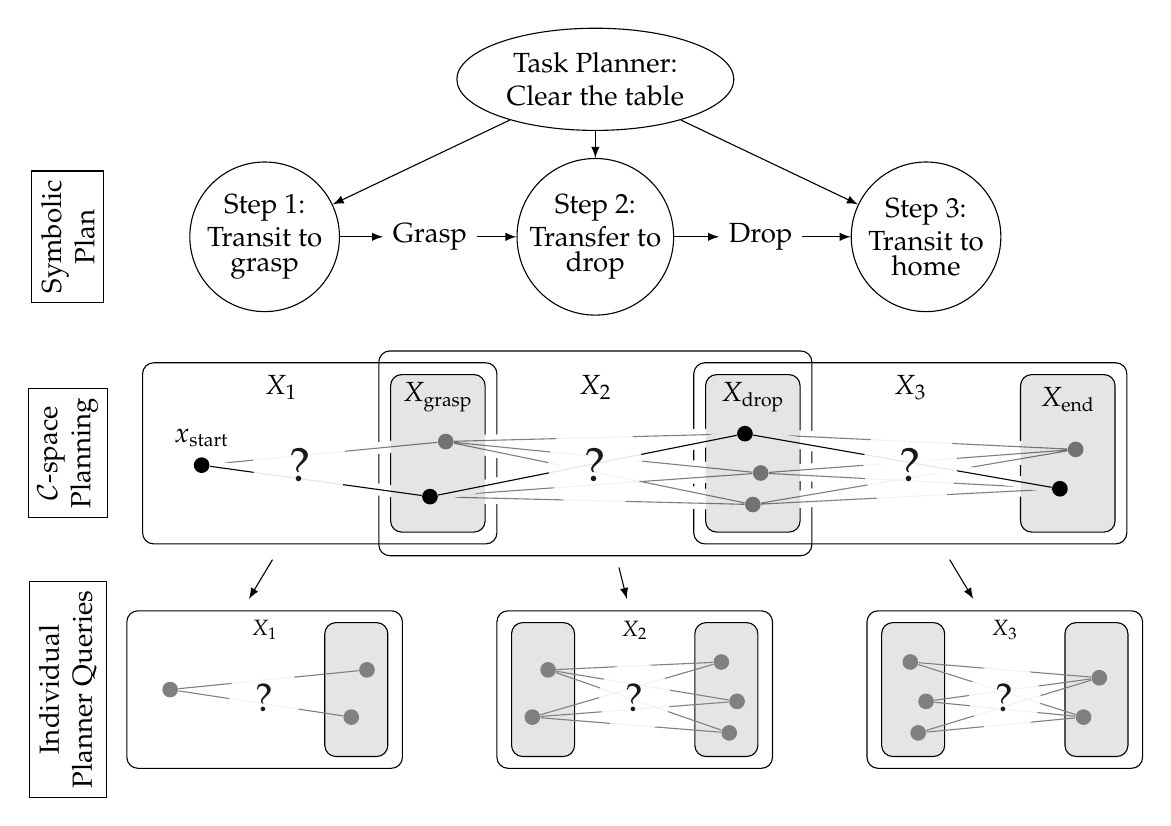
\begin{tikzpicture}
\tikzset{>=latex} % arrow heads

% top: symbolic planner
\node[draw,ellipse,align=center] (high) at (0,0)
   {Task Planner:\\Clear the table};
\node[draw,circle,align=center,inner sep=0,minimum size=1.9cm]
   (step1) at (-4.2,-2)
   {Step 1:\\Transit to\\[-0.04in]grasp};
\node (grasp) at (-2.1,-2) {Grasp};
\node[draw,circle,align=center,inner sep=0,minimum size=1.9cm]
   (step2) at (0,-2)
   {Step 2:\\Transfer to\\[-0.04in]drop};
\node (drop) at (2.1,-2) {Drop};
\node[draw,circle,align=center,inner sep=0,minimum size=1.9cm]
   (step3) at (4.2,-2)
   {Step 3:\\Transit to\\[-0.04in]home};
\draw[->] (high) -- (step1);
\draw[->] (high) -- (step2);
\draw[->] (high) -- (step3);
\draw[->] (step1) -- (grasp);
\draw[->] (grasp) -- (step2);
\draw[->] (step2) -- (drop);
\draw[->] (drop) -- (step3);

% middle: c-space sequence
% valid subsets
\node[draw,black,rounded corners,
   minimum height=2.3cm,minimum width=4.5cm]
   (X1) at (-3.5,-4.75) {};
\node[draw,black,rounded corners,
   minimum height=2.6cm,minimum width=5.5cm]
   (X2) at (0,-4.75) {};
\node[draw,black,rounded corners,
   minimum height=2.3cm,minimum width=5.5cm]
   (X3) at ( 4,-4.75) {};
% root sets
\node[draw,black,rounded corners,
   minimum height=2cm,minimum width=1.2cm]
   (Xgrasp) at (-2,-4.75) {};
\node[draw,black,rounded corners,
   minimum height=2cm,minimum width=1.2cm]
   (Xdrop) at (2,-4.75) {};
\node[draw,black,rounded corners,
   minimum height=2cm,minimum width=1.2cm]
   (Xend) at (6,-4.75) {};
% set labels
\node[above=-0.6cm of Xgrasp] {$X_{\mbox{\scriptsize grasp}}$};
\node[above=-0.6cm of Xdrop] {$X_{\mbox{\scriptsize drop}}$};
\node[above=-0.6cm of Xend] {$X_{\mbox{\scriptsize end}}$};
\node[above left=-0.6cm and -2.1cm of X1] {$X_1$};
\node[above=-0.75cm of X2] {$X_2$};
\node[above=-0.6cm of X3] {$X_3$};
% nodes and paths
\node[circle,fill=black,inner sep=2] (xstart) at (-5,-4.9) {};
\node[circle,fill=black!50,inner sep=2] (xg1) at (-1.9,-4.6) {};
\node[circle,fill=black,inner sep=2] (xg2) at (-2.1,-5.3) {};
\node[circle,fill=black,inner sep=2] (xd1) at ( 1.9,-4.5) {};
\node[circle,fill=black!50,inner sep=2] (xd2) at ( 2.1,-5.0) {};
\node[circle,fill=black!50,inner sep=2] (xd3) at ( 2.0,-5.4) {};
\node[circle,fill=black!50,inner sep=2] (xe1) at ( 6.1,-4.7) {};
\node[circle,fill=black,inner sep=2] (xe2) at ( 5.9,-5.2) {};
\node[above=0cm of xstart] {$x_{\mbox{\scriptsize start}}$};
% lines
\draw[line width=1.5mm,white]
   (xstart) -- (xg1) (xg1) -- (xd1) (xg1) -- (xd2) (xg1) -- (xd3)
   (xg2) -- (xd2) (xg2) -- (xd3) (xd1) -- (xe1) (xd2) -- (xe1)
   (xd2) -- (xe2) (xd3) -- (xe1) (xd3) -- (xe2);
\draw[draw=black!50]
   (xstart) -- (xg1) (xg1) -- (xd1) (xg1) -- (xd2) (xg1) -- (xd3)
   (xg2) -- (xd2) (xg2) -- (xd3) (xd1) -- (xe1) (xd2) -- (xe1)
   (xd2) -- (xe2) (xd3) -- (xe1) (xd3) -- (xe2);
\draw[line width=1.5mm,white]
   (xstart) -- (xg2) (xg2) -- (xd1) (xd1) -- (xe2);
\draw
   (xstart) -- (xg2) (xg2) -- (xd1) (xd1) -- (xe2);
% grey sets (overlay)
\node[fill=black,opacity=0.1,rounded corners,
   minimum height=2cm,minimum width=1.2cm]
   at (-2,-4.75) {};
\node[fill=black,opacity=0.1,rounded corners,
   minimum height=2cm,minimum width=1.2cm]
   at (2,-4.75) {};
\node[fill=black,opacity=0.1,rounded corners,
   minimum height=2cm,minimum width=1.2cm]
   at (6,-4.75) {};
% question mark bubbles
\node[circle,fill=white,fill opacity=0.9,inner sep=7pt]
   at (-3.75,-4.9) {\LARGE ?};
\node[circle,fill=white,fill opacity=0.9,inner sep=7pt]
   at (0,-4.9) {\LARGE ?};
\node[circle,fill=white,fill opacity=0.9,inner sep=7pt]
   at (4.0,-4.9) {\LARGE ?};

% bottom: individual planner instances
\node[draw,black,rounded corners,
   minimum height=2cm,minimum width=3.5cm]
   (sm1) at (-4.2,-7.75) {};
\node[draw,black,fill=black!10,rounded corners,
   minimum height=1.7cm,minimum width=0.8cm,
   right=-1cm of sm1] {};
\node[circle,fill=black!50,inner sep=2] (sm1xstart) at (-5.4,-7.75) {};
\node[circle,fill=black!50,inner sep=2] (sm1xg1) at (-2.9,-7.5) {};
\node[circle,fill=black!50,inner sep=2] (sm1xg2) at (-3.1,-8.1) {};
\draw[draw=black!50]
   (sm1xstart) -- (sm1xg1) (sm1xstart) -- (sm1xg2);
\node[above=-0.5cm of sm1] {\footnotesize $X_1$};
\node[circle,fill=white,fill opacity=0.9,inner sep=5pt]
   at (-4.2,-7.85) {\Large ?};

\node[draw,black,rounded corners,
   minimum height=2cm,minimum width=3.5cm]
   (sm2) at (0.5,-7.75) {};
\node[draw,black,fill=black!10,rounded corners,
   minimum height=1.7cm,minimum width=0.8cm,
   left=-1cm of sm2] {};
\node[draw,black,fill=black!10,rounded corners,
   minimum height=1.7cm,minimum width=0.8cm,
   right=-1cm of sm2] {};
\node[circle,fill=black!50,inner sep=2] (sm2xg1) at (-0.6,-7.5) {};
\node[circle,fill=black!50,inner sep=2] (sm2xg2) at (-0.8,-8.1) {};
\node[circle,fill=black!50,inner sep=2] (sm2xd1) at ( 1.6,-7.4) {};
\node[circle,fill=black!50,inner sep=2] (sm2xd2) at ( 1.8,-7.9) {};
\node[circle,fill=black!50,inner sep=2] (sm2xd3) at ( 1.7,-8.3) {};
\draw[draw=black!50]
   (sm2xg1) -- (sm2xd1) (sm2xg1) -- (sm2xd2) (sm2xg1) -- (sm2xd3)
   (sm2xg2) -- (sm2xd1) (sm2xg2) -- (sm2xd2) (sm2xg2) -- (sm2xd3);
\node[above=-0.5cm of sm2] {\footnotesize $X_2$};
\node[circle,fill=white,fill opacity=0.9,inner sep=5pt]
   at (0.5,-7.85) {\Large ?};

\node[draw,black,rounded corners,
   minimum height=2cm,minimum width=3.5cm]
   (sm3) at (5.2,-7.75) {};
\node[draw,black,fill=black!10,rounded corners,
   minimum height=1.7cm,minimum width=0.8cm,
   left=-1cm of sm3] {};
\node[draw,black,fill=black!10,rounded corners,
   minimum height=1.7cm,minimum width=0.8cm,
   right=-1cm of sm3] {};
\node[circle,fill=black!50,inner sep=2] (sm3xd1) at ( 4.0,-7.4) {};
\node[circle,fill=black!50,inner sep=2] (sm3xd2) at ( 4.2,-7.9) {};
\node[circle,fill=black!50,inner sep=2] (sm3xd3) at ( 4.1,-8.3) {};
\node[circle,fill=black!50,inner sep=2] (sm3xe1) at ( 6.4,-7.6) {};
\node[circle,fill=black!50,inner sep=2] (sm3xe2) at ( 6.2,-8.1) {};
\draw[draw=black!50]
   (sm3xd1) -- (sm3xe1) (sm3xd1) -- (sm3xe2) (sm3xd2) -- (sm3xe1)
   (sm3xd2) -- (sm3xe2) (sm3xd3) -- (sm3xe1) (sm3xd3) -- (sm3xe2);
\node[above=-0.5cm of sm3] {\footnotesize $X_3$};
\node[circle,fill=white,fill opacity=0.9,inner sep=5pt]
   at (5.2,-7.85) {\Large ?};

% arrows
\draw[->] (-4.1,-6.1) -- (-4.4,-6.6);
\draw[->] ( 0.3,-6.2) -- ( 0.4,-6.6);
\draw[->] ( 4.5,-6.1) -- ( 4.8,-6.6);

% side labels
\node[draw,rotate=90,align=center] at (-6.7,-2)
   {Symbolic\\Plan};
\node[draw,rotate=90,align=center] at (-6.7,-4.75)
   {$\mathcal{C}$-space\\Planning};
\node[draw,rotate=90,align=center] at (-6.7,-7.75)
   {Individual\\Planner Queries};

\end{tikzpicture}%
\end{document}
